\documentclass[twoside]{book}

% Packages required by doxygen
\usepackage{fixltx2e}
\usepackage{calc}
\usepackage{doxygen}
\usepackage[export]{adjustbox} % also loads graphicx
\usepackage{graphicx}
\usepackage[utf8]{inputenc}
\usepackage{makeidx}
\usepackage{multicol}
\usepackage{multirow}
\PassOptionsToPackage{warn}{textcomp}
\usepackage{textcomp}
\usepackage[nointegrals]{wasysym}
\usepackage[table]{xcolor}

% Font selection
\usepackage[T1]{fontenc}
\usepackage[scaled=.90]{helvet}
\usepackage{courier}
\usepackage{amssymb}
\usepackage{sectsty}
\renewcommand{\familydefault}{\sfdefault}
\allsectionsfont{%
  \fontseries{bc}\selectfont%
  \color{darkgray}%
}
\renewcommand{\DoxyLabelFont}{%
  \fontseries{bc}\selectfont%
  \color{darkgray}%
}
\newcommand{\+}{\discretionary{\mbox{\scriptsize$\hookleftarrow$}}{}{}}

% Page & text layout
\usepackage{geometry}
\geometry{%
  a4paper,%
  top=2.5cm,%
  bottom=2.5cm,%
  left=2.5cm,%
  right=2.5cm%
}
\tolerance=750
\hfuzz=15pt
\hbadness=750
\setlength{\emergencystretch}{15pt}
\setlength{\parindent}{0cm}
\setlength{\parskip}{0.2cm}
\makeatletter
\renewcommand{\paragraph}{%
  \@startsection{paragraph}{4}{0ex}{-1.0ex}{1.0ex}{%
    \normalfont\normalsize\bfseries\SS@parafont%
  }%
}
\renewcommand{\subparagraph}{%
  \@startsection{subparagraph}{5}{0ex}{-1.0ex}{1.0ex}{%
    \normalfont\normalsize\bfseries\SS@subparafont%
  }%
}
\makeatother

% Headers & footers
\usepackage{fancyhdr}
\pagestyle{fancyplain}
\fancyhead[LE]{\fancyplain{}{\bfseries\thepage}}
\fancyhead[CE]{\fancyplain{}{}}
\fancyhead[RE]{\fancyplain{}{\bfseries\leftmark}}
\fancyhead[LO]{\fancyplain{}{\bfseries\rightmark}}
\fancyhead[CO]{\fancyplain{}{}}
\fancyhead[RO]{\fancyplain{}{\bfseries\thepage}}
\fancyfoot[LE]{\fancyplain{}{}}
\fancyfoot[CE]{\fancyplain{}{}}
\fancyfoot[RE]{\fancyplain{}{\bfseries\scriptsize Generated on Mon Nov 16 2015 23\+:24\+:00 for Item\+Prototype by Doxygen }}
\fancyfoot[LO]{\fancyplain{}{\bfseries\scriptsize Generated on Mon Nov 16 2015 23\+:24\+:00 for Item\+Prototype by Doxygen }}
\fancyfoot[CO]{\fancyplain{}{}}
\fancyfoot[RO]{\fancyplain{}{}}
\renewcommand{\footrulewidth}{0.4pt}
\renewcommand{\chaptermark}[1]{%
  \markboth{#1}{}%
}
\renewcommand{\sectionmark}[1]{%
  \markright{\thesection\ #1}%
}

% Indices & bibliography
\usepackage{natbib}
\usepackage[titles]{tocloft}
\setcounter{tocdepth}{3}
\setcounter{secnumdepth}{5}
\makeindex

% Hyperlinks (required, but should be loaded last)
\usepackage{ifpdf}
\ifpdf
  \usepackage[pdftex,pagebackref=true]{hyperref}
\else
  \usepackage[ps2pdf,pagebackref=true]{hyperref}
\fi
\hypersetup{%
  colorlinks=true,%
  linkcolor=blue,%
  citecolor=blue,%
  unicode%
}

% Custom commands
\newcommand{\clearemptydoublepage}{%
  \newpage{\pagestyle{empty}\cleardoublepage}%
}


%===== C O N T E N T S =====

\begin{document}

% Titlepage & ToC
\hypersetup{pageanchor=false,
             bookmarks=true,
             bookmarksnumbered=true,
             pdfencoding=unicode
            }
\pagenumbering{roman}
\begin{titlepage}
\vspace*{7cm}
\begin{center}%
{\Large Item\+Prototype }\\
\vspace*{1cm}
{\large Generated by Doxygen 1.8.10}\\
\vspace*{0.5cm}
{\small Mon Nov 16 2015 23:24:00}\\
\end{center}
\end{titlepage}
\clearemptydoublepage
\tableofcontents
\clearemptydoublepage
\pagenumbering{arabic}
\hypersetup{pageanchor=true}

%--- Begin generated contents ---
\chapter{Hierarchical Index}
\section{Class Hierarchy}
This inheritance list is sorted roughly, but not completely, alphabetically\+:\begin{DoxyCompactList}
\item \contentsline{section}{Item}{\pageref{class_item}}{}
\begin{DoxyCompactList}
\item \contentsline{section}{Antidote}{\pageref{class_antidote}}{}
\item \contentsline{section}{Potion}{\pageref{class_potion}}{}
\end{DoxyCompactList}
\item \contentsline{section}{Item\+Factory}{\pageref{class_item_factory}}{}
\end{DoxyCompactList}

\chapter{Class Index}
\section{Class List}
Here are the classes, structs, unions and interfaces with brief descriptions\+:\begin{DoxyCompactList}
\item\contentsline{section}{\hyperlink{class_antidote}{Antidote} \\*An \hyperlink{class_antidote}{Antidote} class }{\pageref{class_antidote}}{}
\item\contentsline{section}{\hyperlink{class_item}{Item} \\*Abstract \hyperlink{class_item}{Item} Class }{\pageref{class_item}}{}
\item\contentsline{section}{\hyperlink{class_item_factory}{Item\+Factory} \\*An \hyperlink{class_item_factory}{Item\+Factory} class }{\pageref{class_item_factory}}{}
\item\contentsline{section}{\hyperlink{class_potion}{Potion} \\*A \hyperlink{class_potion}{Potion} class inherited from \hyperlink{class_item}{Item} class }{\pageref{class_potion}}{}
\end{DoxyCompactList}

\chapter{Class Documentation}
\hypertarget{class_antidote}{}\section{Antidote Class Reference}
\label{class_antidote}\index{Antidote@{Antidote}}


An \hyperlink{class_antidote}{Antidote} class.  




{\ttfamily \#include $<$Item\+Prototype.\+h$>$}

Inheritance diagram for Antidote\+:\begin{figure}[H]
\begin{center}
\leavevmode
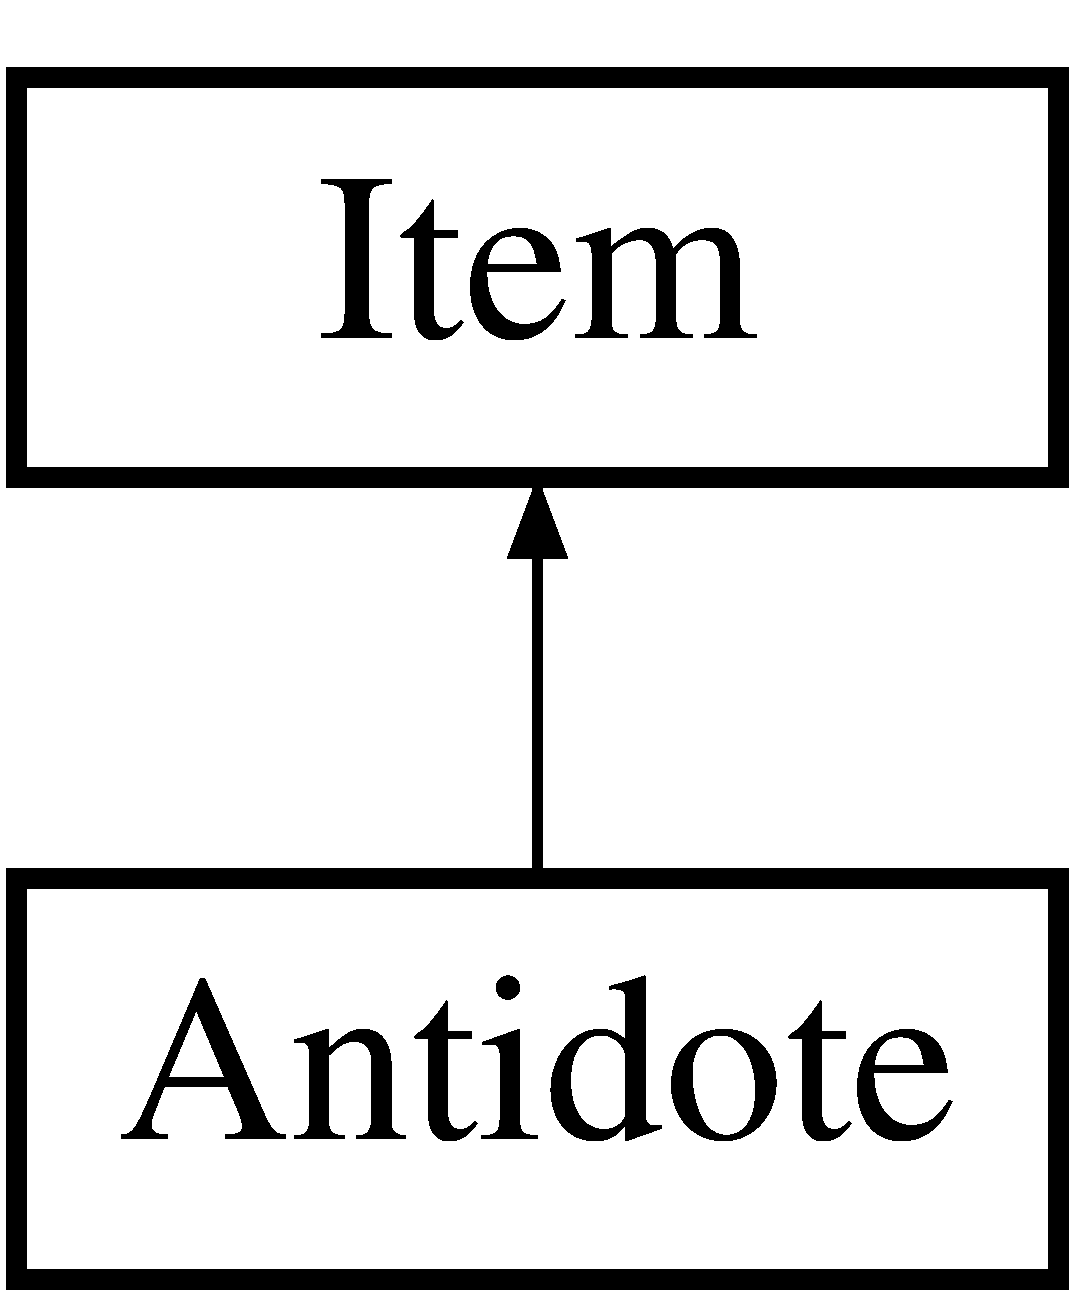
\includegraphics[height=2.000000cm]{class_antidote}
\end{center}
\end{figure}
\subsection*{Public Member Functions}
\begin{DoxyCompactItemize}
\item 
\hypertarget{class_antidote_af9e842ead3c6fbab1147056647ec0ced}{}\hyperlink{class_antidote_af9e842ead3c6fbab1147056647ec0ced}{Antidote} (string name)\label{class_antidote_af9e842ead3c6fbab1147056647ec0ced}

\begin{DoxyCompactList}\small\item\em Constructs an object \hyperlink{class_antidote}{Antidote}. \end{DoxyCompactList}\item 
\hypertarget{class_antidote_af984adccc80a2f49791d6bdfd4918201}{}\hyperlink{class_item}{Item} $\ast$ \hyperlink{class_antidote_af984adccc80a2f49791d6bdfd4918201}{clone} (string name)\label{class_antidote_af984adccc80a2f49791d6bdfd4918201}

\begin{DoxyCompactList}\small\item\em Return a new object \hyperlink{class_antidote}{Antidote}. \end{DoxyCompactList}\end{DoxyCompactItemize}
\subsection*{Additional Inherited Members}


\subsection{Detailed Description}
An \hyperlink{class_antidote}{Antidote} class. 

\hyperlink{class_antidote}{Antidote} class inherited from \hyperlink{class_item}{Item} class. It contains a constructor and a clone function. It is used to cure the player from poison. 

The documentation for this class was generated from the following files\+:\begin{DoxyCompactItemize}
\item 
C\+:/\+Users/\+Mook T/\+Desktop/item/Item\+Prototype.\+h\item 
C\+:/\+Users/\+Mook T/\+Desktop/item/Item\+Prototype.\+cpp\end{DoxyCompactItemize}

\hypertarget{class_item}{}\section{Item Class Reference}
\label{class_item}\index{Item@{Item}}


Abstract \hyperlink{class_item}{Item} Class.  




{\ttfamily \#include $<$Item\+Prototype.\+h$>$}

Inheritance diagram for Item\+:\begin{figure}[H]
\begin{center}
\leavevmode
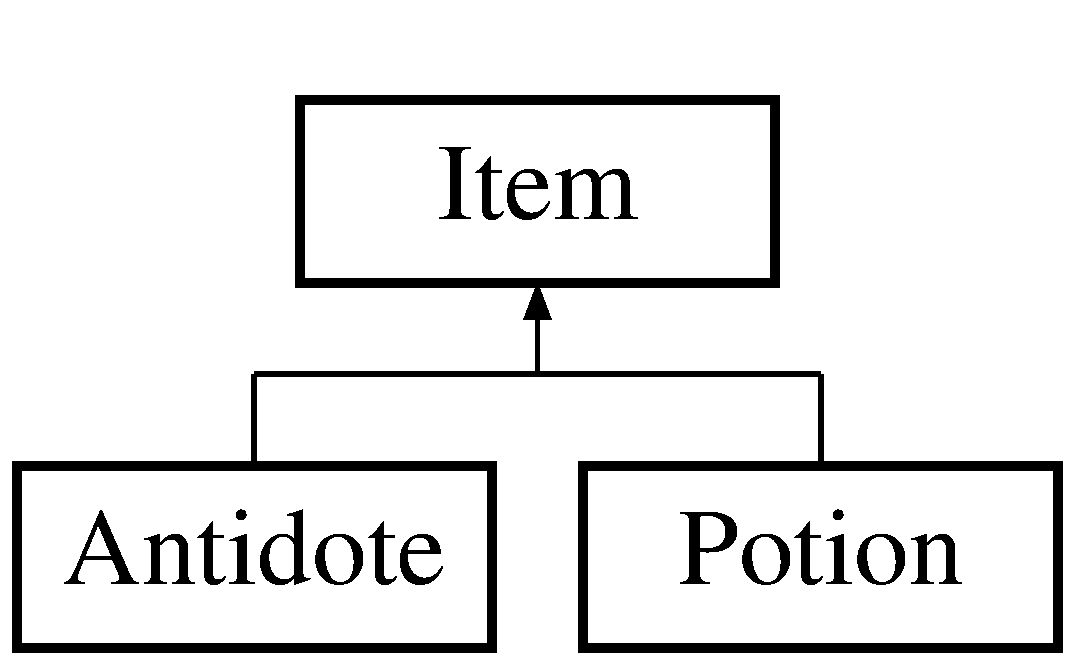
\includegraphics[height=2.000000cm]{class_item}
\end{center}
\end{figure}
\subsection*{Public Member Functions}
\begin{DoxyCompactItemize}
\item 
\hypertarget{class_item_aee86b49539ec0027b06b5c703e386de8}{}virtual \hyperlink{class_item}{Item} $\ast$ \hyperlink{class_item_aee86b49539ec0027b06b5c703e386de8}{clone} (string name)=0\label{class_item_aee86b49539ec0027b06b5c703e386de8}

\begin{DoxyCompactList}\small\item\em Pure virtual clone method. \end{DoxyCompactList}\item 
\hypertarget{class_item_ad3c548eb69bdb99ccbe41bdad8e4eb41}{}void \hyperlink{class_item_ad3c548eb69bdb99ccbe41bdad8e4eb41}{print\+Item} ()\label{class_item_ad3c548eb69bdb99ccbe41bdad8e4eb41}

\begin{DoxyCompactList}\small\item\em Print out statement confirming object has been created. \end{DoxyCompactList}\item 
\hypertarget{class_item_a2aea1cc560205b01eaf5250c21f4fc71}{}string \hyperlink{class_item_a2aea1cc560205b01eaf5250c21f4fc71}{get\+Type} ()\label{class_item_a2aea1cc560205b01eaf5250c21f4fc71}

\begin{DoxyCompactList}\small\item\em Return the type of the object. \end{DoxyCompactList}\item 
\hypertarget{class_item_a63d7f2148b699e539aae354b01559811}{}string \hyperlink{class_item_a63d7f2148b699e539aae354b01559811}{get\+Name} ()\label{class_item_a63d7f2148b699e539aae354b01559811}

\begin{DoxyCompactList}\small\item\em Return the name of the object. \end{DoxyCompactList}\item 
\hypertarget{class_item_a70ce365b03e94a33d4a137dcd9fa2818}{}\hyperlink{class_json_1_1_value}{Json\+::\+Value} \hyperlink{class_item_a70ce365b03e94a33d4a137dcd9fa2818}{to\+Json} () const \label{class_item_a70ce365b03e94a33d4a137dcd9fa2818}

\begin{DoxyCompactList}\small\item\em creating a J\+S\+O\+N object \end{DoxyCompactList}\end{DoxyCompactItemize}
\subsection*{Protected Attributes}
\begin{DoxyCompactItemize}
\item 
\hypertarget{class_item_a1b0c64bfa9407d49b5ad91d6a7372a38}{}string \hyperlink{class_item_a1b0c64bfa9407d49b5ad91d6a7372a38}{item\+Type}\label{class_item_a1b0c64bfa9407d49b5ad91d6a7372a38}

\begin{DoxyCompactList}\small\item\em Store the type of the object. \end{DoxyCompactList}\item 
\hypertarget{class_item_af7a09a8db2072c632d84a992e76408b9}{}string \hyperlink{class_item_af7a09a8db2072c632d84a992e76408b9}{item\+Name}\label{class_item_af7a09a8db2072c632d84a992e76408b9}

\begin{DoxyCompactList}\small\item\em Store the name of the object. \end{DoxyCompactList}\end{DoxyCompactItemize}


\subsection{Detailed Description}
Abstract \hyperlink{class_item}{Item} Class. 

The documentation for this class was generated from the following files\+:\begin{DoxyCompactItemize}
\item 
C\+:/\+Users/\+Mook T/\+Desktop/item/Item\+Prototype.\+h\item 
C\+:/\+Users/\+Mook T/\+Desktop/item/Item\+Prototype.\+cpp\end{DoxyCompactItemize}

\hypertarget{class_item_factory}{}\section{Item\+Factory Class Reference}
\label{class_item_factory}\index{Item\+Factory@{Item\+Factory}}


An \hyperlink{class_item_factory}{Item\+Factory} class.  




{\ttfamily \#include $<$Item\+Prototype.\+h$>$}

\subsection*{Static Public Member Functions}
\begin{DoxyCompactItemize}
\item 
\hypertarget{class_item_factory_a7c6bdc209944c5b0e6a98da6434ef1f7}{}static void \hyperlink{class_item_factory_a7c6bdc209944c5b0e6a98da6434ef1f7}{initialize} ()\label{class_item_factory_a7c6bdc209944c5b0e6a98da6434ef1f7}

\begin{DoxyCompactList}\small\item\em Initialized the prototypes. \end{DoxyCompactList}\item 
\hypertarget{class_item_factory_a47e59f627e5a3ab710138ae6f1c7e6da}{}static \hyperlink{class_item}{Item} $\ast$ \hyperlink{class_item_factory_a47e59f627e5a3ab710138ae6f1c7e6da}{make\+Potion} (string name)\label{class_item_factory_a47e59f627e5a3ab710138ae6f1c7e6da}

\begin{DoxyCompactList}\small\item\em Call the clone() of \hyperlink{class_potion}{Potion} and return the object. \end{DoxyCompactList}\item 
\hypertarget{class_item_factory_a0ece2a36df02fa03f27bf99f145b9019}{}static \hyperlink{class_item}{Item} $\ast$ \hyperlink{class_item_factory_a0ece2a36df02fa03f27bf99f145b9019}{make\+Antidote} (string name)\label{class_item_factory_a0ece2a36df02fa03f27bf99f145b9019}

\begin{DoxyCompactList}\small\item\em Call the clone() of \hyperlink{class_antidote}{Antidote} and return the object. \end{DoxyCompactList}\end{DoxyCompactItemize}
\subsection*{Static Public Attributes}
\begin{DoxyCompactItemize}
\item 
\hypertarget{class_item_factory_a26325ba5225e258360465076f44a8c6c}{}static \hyperlink{class_item}{Item} $\ast$ \hyperlink{class_item_factory_a26325ba5225e258360465076f44a8c6c}{potion} = 0\label{class_item_factory_a26325ba5225e258360465076f44a8c6c}

\begin{DoxyCompactList}\small\item\em A pointer to the \hyperlink{class_potion}{Potion} prototype. \end{DoxyCompactList}\item 
\hypertarget{class_item_factory_aa4b3dbb8ff64d34373907c78a5c6787c}{}static \hyperlink{class_item}{Item} $\ast$ \hyperlink{class_item_factory_aa4b3dbb8ff64d34373907c78a5c6787c}{antidote} = 0\label{class_item_factory_aa4b3dbb8ff64d34373907c78a5c6787c}

\begin{DoxyCompactList}\small\item\em A pointer to the \hyperlink{class_antidote}{Antidote} prototype. \end{DoxyCompactList}\end{DoxyCompactItemize}


\subsection{Detailed Description}
An \hyperlink{class_item_factory}{Item\+Factory} class. 

\hyperlink{class_item_factory}{Item\+Factory} store the prototypes and calls the clone() on that object, and return the object. 

The documentation for this class was generated from the following files\+:\begin{DoxyCompactItemize}
\item 
C\+:/\+Users/\+Mook T/\+Desktop/item/Item\+Prototype.\+h\item 
C\+:/\+Users/\+Mook T/\+Desktop/item/Item\+Prototype.\+cpp\end{DoxyCompactItemize}

\hypertarget{class_potion}{}\section{Potion Class Reference}
\label{class_potion}\index{Potion@{Potion}}


A \hyperlink{class_potion}{Potion} class inherited from \hyperlink{class_item}{Item} class.  




{\ttfamily \#include $<$Item\+Prototype.\+h$>$}

Inheritance diagram for Potion\+:\begin{figure}[H]
\begin{center}
\leavevmode
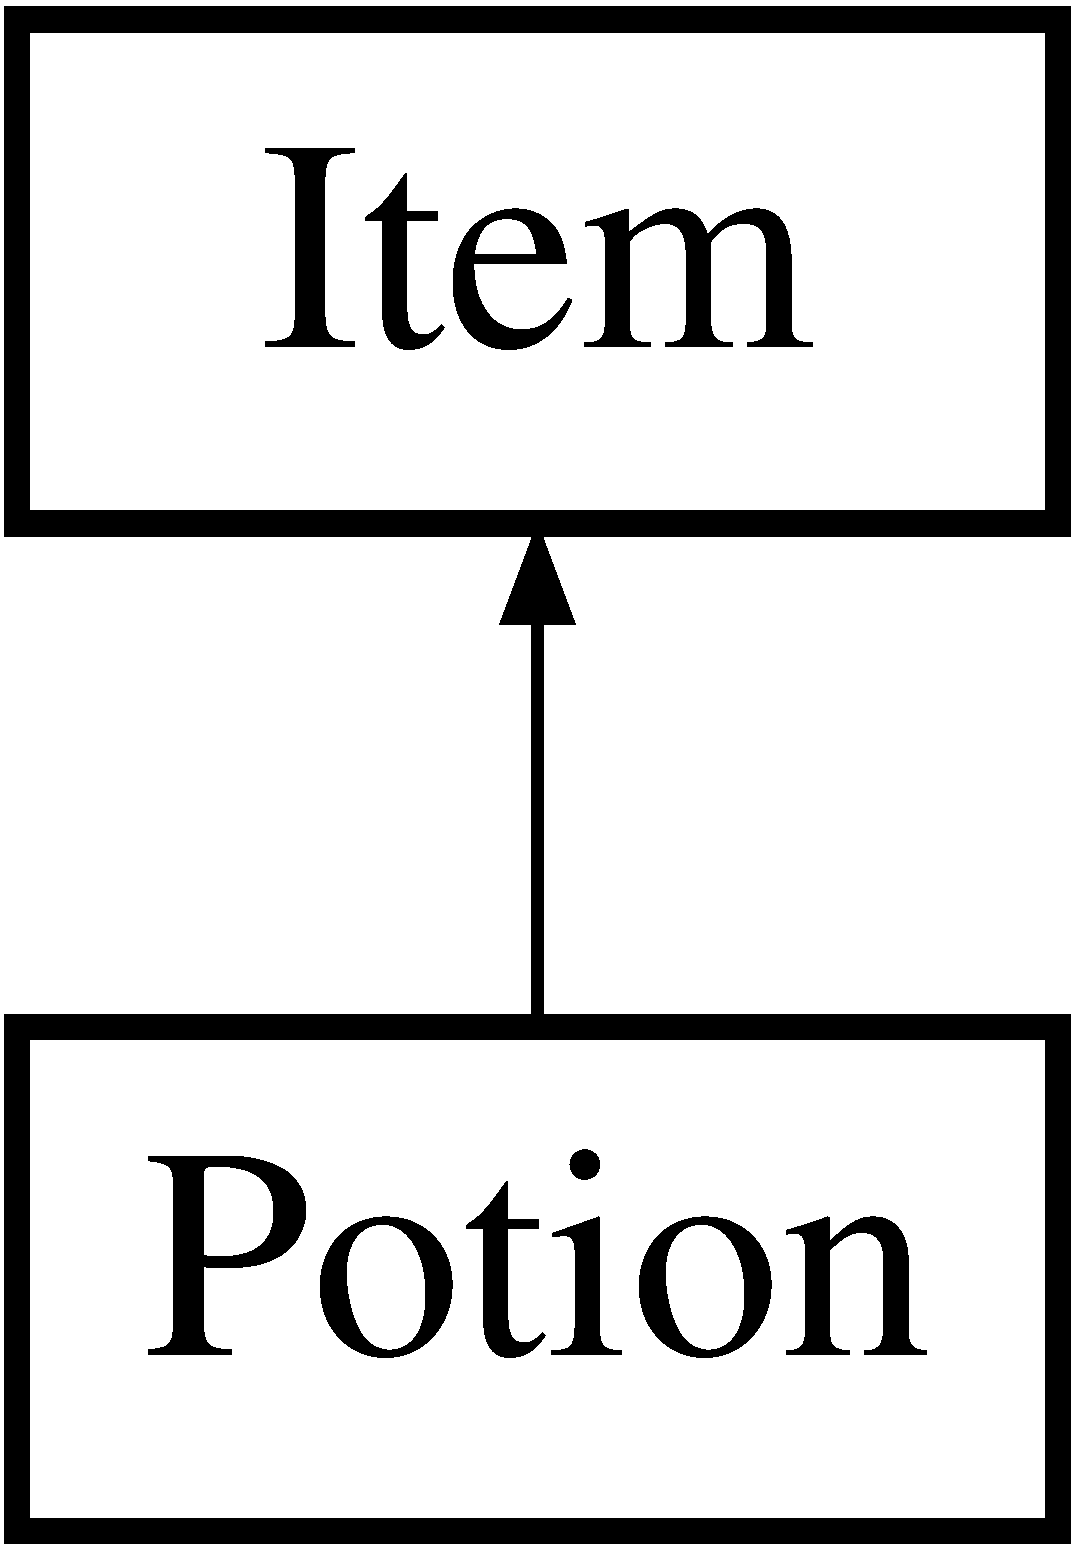
\includegraphics[height=2.000000cm]{class_potion}
\end{center}
\end{figure}
\subsection*{Public Member Functions}
\begin{DoxyCompactItemize}
\item 
\hypertarget{class_potion_ae85fd98bf8c9da25af439bac1581edf4}{}\hyperlink{class_potion_ae85fd98bf8c9da25af439bac1581edf4}{Potion} (string name)\label{class_potion_ae85fd98bf8c9da25af439bac1581edf4}

\begin{DoxyCompactList}\small\item\em Constructs an object \hyperlink{class_potion}{Potion}. \end{DoxyCompactList}\item 
\hypertarget{class_potion_a79ea83f8d6cd83dcfb8bae13760684a8}{}\hyperlink{class_item}{Item} $\ast$ \hyperlink{class_potion_a79ea83f8d6cd83dcfb8bae13760684a8}{clone} (string name)\label{class_potion_a79ea83f8d6cd83dcfb8bae13760684a8}

\begin{DoxyCompactList}\small\item\em Return a new object \hyperlink{class_potion}{Potion}. \end{DoxyCompactList}\end{DoxyCompactItemize}
\subsection*{Additional Inherited Members}


\subsection{Detailed Description}
A \hyperlink{class_potion}{Potion} class inherited from \hyperlink{class_item}{Item} class. 

\hyperlink{class_potion}{Potion} class inherited from \hyperlink{class_item}{Item} class. It contains a constructor and a clone function. It is used to increase the player\textquotesingle{}s health. 

The documentation for this class was generated from the following files\+:\begin{DoxyCompactItemize}
\item 
C\+:/\+Users/\+Mook T/\+Desktop/item/Item\+Prototype.\+h\item 
C\+:/\+Users/\+Mook T/\+Desktop/item/Item\+Prototype.\+cpp\end{DoxyCompactItemize}

%--- End generated contents ---

% Index
\backmatter
\newpage
\phantomsection
\clearemptydoublepage
\addcontentsline{toc}{chapter}{Index}
\printindex

\end{document}
